\chapter{W�nsche an FAS}
\label{W�nsche}

\begin{itemize}

\item \textbf{Bekanntgabe}\\
Per E-Mail, Telefonanruf auf der FAS-Hotline -222 oder pers�nlich bei einem der Mitarbeiter des FAS-Online Projekts.

\item \textbf{Wunschliste}\\
Die W�nsche werden auf einer Liste gesammelt.

\item \textbf{Aufwandsch�tzung}\\
Entweder wird der Wunsch gleich in die ToDo-Liste gereiht oder es werden im FAS-Meeting allf�llige Fragen gekl�rt.
Eventuell wird hier auch eine Arbeitsgruppe gebildet, um den Wunsch auszuarbeiten.

\item \textbf{Priorisierung}\\
Die ToDo-Liste wird im FAS-Meeting nach Wichtigkeit priorisiert.

\end{itemize}


\begin {figure}
	\centering
	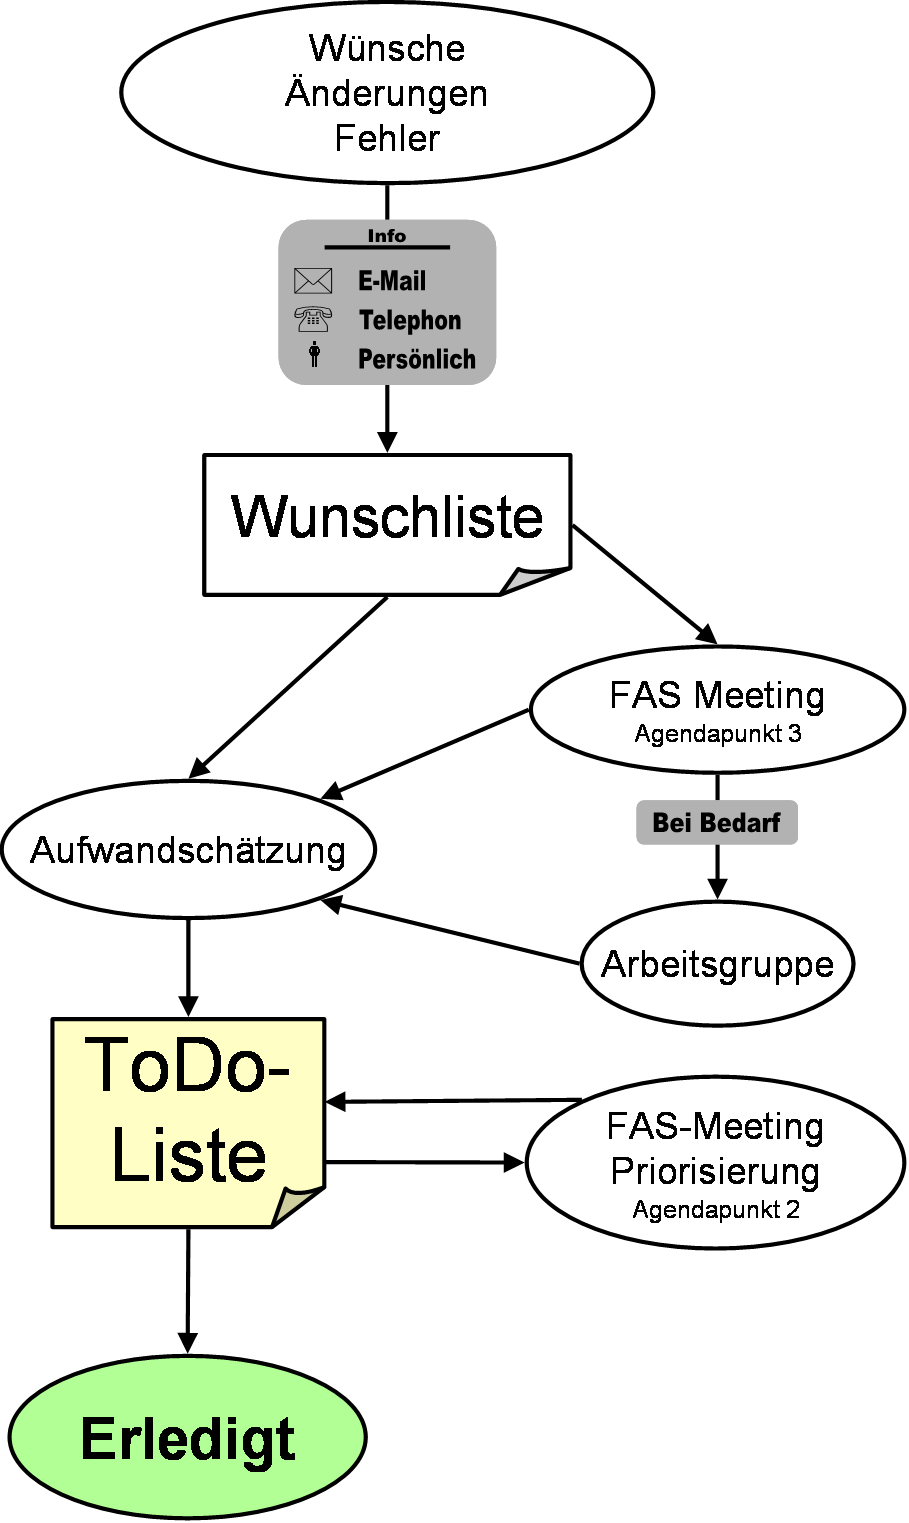
\includegraphics[height=110mm]{Prozess_FAS-Meeting}
	\caption{Prozessdiagramm eines Wunsches ans FAS}
	\label{Prozess}
\end {figure}


%\section{Hauptmen�}
%
\includegraphics{eins}
%Im Hauptmen� k�nnen Sie die grundlegenden Einstellungen vornehmen.
%Im Punkt ''Einstellungen'' w�hlen Sie das Studiensemester, das Sie bearbeiten m�chten.
%Hier k�nnen Sie auch auf die Onlinetabelle (Stundenplan) wechseln, in der �nderungen sofort auf dem Studentenplan sichtbar werden.
%Au�erdem k�nnen Sie hier die drei verschiedenen Kollisions�berpr�fungen aktivieren und deaktivieren. (siehe Kapitel \ref{Kapitel Kollisionen})

%\info{Das aktuell eingestellte Studiensemester und die aktuell aktive Datenbanktabelle werden im Fenster ganz links unten angezeigt.}

%\section{Quellmen�}
%
\includegraphics{zwei}
%Hier k�nnen Sie zwischen dem Lehrverband, dem Ort und dem Lektor w�hlen, 
%welcher im Hauptfenster (4) angezeigt werden soll.
%Das Quellmen� ist als Baumstruktur aufgebaut. Durch Klicken auf die kleinen Pfeile blenden Sie eine untergeordnete Gruppe ein und k�nnen diese damit auch wieder ausblenden.
%Eine ausgew�hlte Zeile wird \colorbox{yellow}{gelb} markiert, was sich auch nach Wechsel des Karteireiters nicht �ndert. Der Inhalt des Hauptfensters wird an die gew�hlte Zeile angepasst.

%\info{Wenn Sie den Karteireiter im Quellmen� wechseln und wiederholt einen anderen Karteireiter aufrufen, m�ssen Sie erneut auf die gelb unterlegte Zeile klicken, um die Ansicht im Hauptfenster zu aktualisieren.}

%\idee{TIPP	Sie brauchen nicht die lange Liste an Lektoren h�ndisch durchscrollen. Markieren Sie einen beliebigen Lektor und geben Sie den Namen des gesuchten Lektors auf der Tastatur ein.}

%
\includegraphics{Listenfeld_ConfigButton}...Dieser Button blendet zus�tzliche Details im jeweiligen Karteireiter ein.

%\section{Ansicht}
%
\includegraphics{drei}
%W�hlen Sie hier die Ansicht, die im Hauptfenster dargestellt werden soll.
%Beim Start wird standardm��ig der Wochenplan aus der aktuellen Kalenderwoche angezeigt.

%Die Ansicht ist an das Quellmen� gekoppelt.
%Um beispielsweise den entsprechenden Studiengang in der Registerkarte ''Wochenplan'' anzeigen zu k�nnen, muss im Quellmen� ein Lehrverband ausgew�hlt werden.

%Die Registerkarten der Ansicht, werden ab Kapitel \ref{Kapitel Semesterplan} n�her beschrieben.
%Die Registerkarte ''Lehrveranstaltung'' wird in Kapitel \ref{Kapitel Lehreinheit} genau behandelt.


%\achtung{Achtung: Es erfolgt dabei KEINE Kollisions�berpr�fung!}


%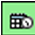
\includegraphics{single_week}...Vorschlag/Setzen SingleWeek:
%Einmaliges verplanen einer Lehreinheit \textit{(in der im Hauptfenster angezeigten Kalenderwoche)}. Ein einmaliger Klick zeigt Raumvorschl�ge unter Ber�cksichtigung der Blockung und etwaiger Kollisionen im Hauptfenster an. Per Drag\&Drop kann die Lehreinheit dann in den gew�nschten Raum gezogen werden und wird dort mit der eingestellten Blockung verplant.\\
